%%%%%%%%%%%%%%%%%%%%%%%%%%%%%%%%%%%%%%%%%%%%%%
%                insertmeeting
% 1) Title (something creative & funny?)
% 2) Date (MM/DD/YYYY)
% 3) Location (ex. Hagerty High School)
% 4) People/Committees Present 
% 5) Picture 
% 6) Start Time & Stop Time (ex. 12:30AM to 4:30PM)
%%%%%%%%%%%%%%%%%%%%%%%%%%%%%%%%%%%%%%%%%%%%%%
\insertmeeting 
	{Froggy Friday} 
	{03/10/22} 
	{Hagerty High School}
	{James, Jensen, Nathan, Ritam}
	{Images/RobotPics/robot.jpg}
	{2:30 - 8:30}
	
\hhscommittee{Software}
\noindent\hfil\rule{\textwidth}{.4pt}\hfil
\subsubsection*{Goals}
\begin{itemize}
    \item Improve arm movement

\end{itemize} 

\noindent\hfil\rule{\textwidth}{.4pt}\hfil

\subsubsection*{Accomplishments}
Heading into States, we were pretty happy with how our arm moved. However, one thing we noticed in the weeks leading up to the competition was the high variability in encoder readings. Using the encoder from a REV Hex motor to control our arm, we were able to move the arm to various positions in code. However, this movement could occasionally come out very jerky. Today, our main goal was to determine the reason behind the inconistent jerks and brainstorm possible solutions. The first thing we did was use the FTC dashboard to graph the output our program was sending to the motor. One thing we noticed from the graph was that even the PID output was very jagged. This suggests that there were issues in the PID calcuation. Deciding to graph the encoder position, we realized that the encoder was sending high-variability measurements. After asking our mentor, he explained that this could be caused by slow reading speed or built-in weaknesses of the encoder. To solve our arm issue, we had to come up with a way to "smooth out" these measurements. Our mentor suggested the use of a simple moving average. Our first implemenation used a fixed length array, moving all the values over one position and discarding the oldest measurement when a new measurement was taken. While we thought that this was working well, we ran into run-time errors during execution of seemingly unreleated autonomous programs. Using Android Studio's logging utility revealed that there was an issue with Java's automated garbage collector, where it paused the program and caused the robot to stall. Our mentor explained to us that an issue could have been caused with the SimpleMovingAverage, where we could have been overloading the system memory and triggering a garbage collector execution. To solve this, we switched to using a circle array method. This implementation took a much longer period of time, but it eventually proved more consistent than our previous methods. 


\begin{figure}[htp]
\centering
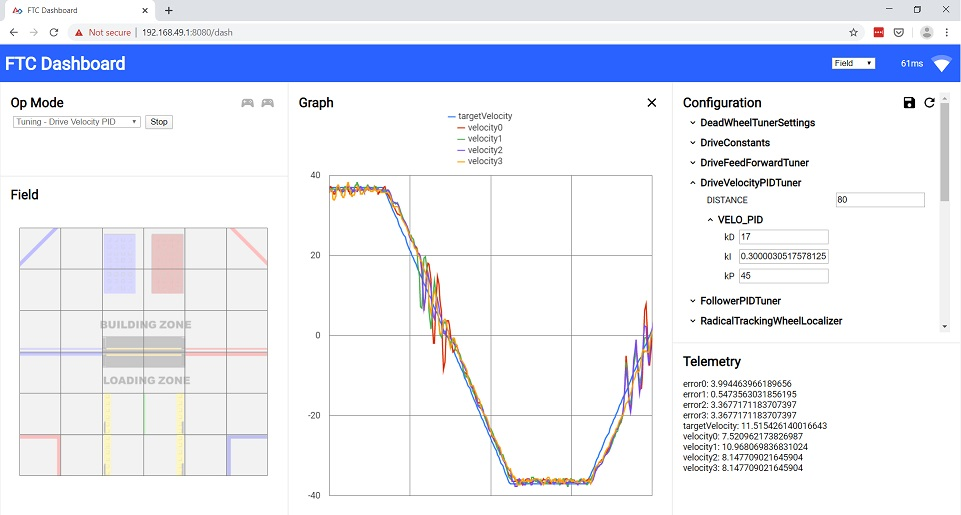
\includegraphics[width=0.95\textwidth, angle=0]{Meetings/March/03-10-22/03-10-22 1.jpg}
\caption{This is a screenshot from the official website for FTC Dashboard, a tool we use to aid our robot development process.}
\label{fig:031022_1}
\end{figure}

\begin{figure}[htp]
\centering
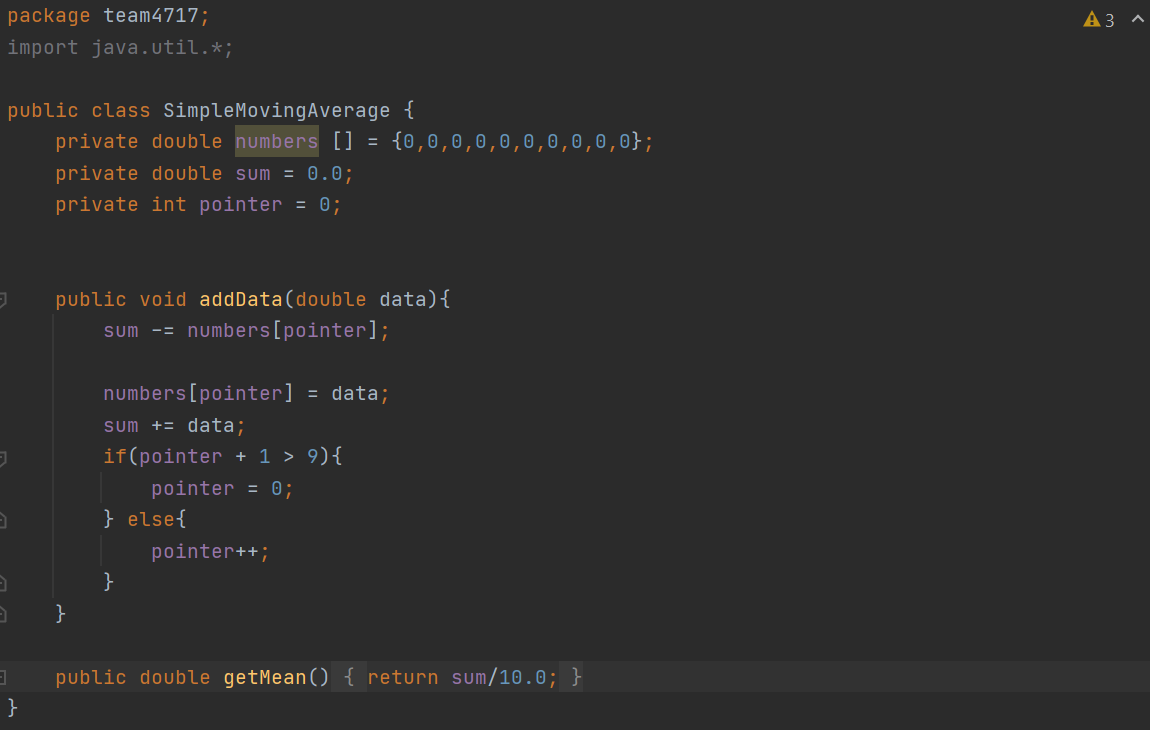
\includegraphics[width=0.95\textwidth, angle=0]{Meetings/March/03-10-22/03-10-22 2.png}
\caption{The working implementation of the SimpleMovingAverage using the circular array implementation.}
\label{fig:031022_2}
\end{figure}

\begin{figure}[htp]
\centering
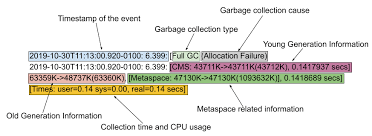
\includegraphics[width=0.95\textwidth, angle=0]{Meetings/March/03-10-22/03-10-22 3.png}
\caption{An example of the output we saw from the Android Studio Logcat.}
\label{fig:031022_3}
\end{figure}




\whatsnext{
\begin{itemize}
    \item Work to improve the autonomous program. 
\end{itemize} 
}

